% Volume III, Chapter 2 (drafted as "Chapter 28")
\chapter{Simplicial Sandpiles on \texorpdfstring{$\Atwo$}{A2} Complexes: Sign Obstructions, Hodge Factorization, and Avalanche Statistics}\label{chap:V3P2}
\chaptermark{Simplicial Sandpiles}
\begin{chapterabstract}
The proposed programme asks for abelian sandpile dynamics on the $k$-simplices of an $\Atwo$
complex, toppled by the Hodge Laplacians $\Delta_k$, for a recurrent-configuration group
$\operatorname{Pic}_k(Y)$, and for critical avalanche exponents on buildings. This chapter
establishes what can be established and says what cannot.

(1) \emph{The sign obstruction.} A threshold rule $z\mapsto z-Me_i$ is an abelian sandpile in
Dhar's sense when $M$ is a Z-matrix, i.e.\ has non-positive off-diagonal entries. We prove
that on every $\Atwo$ complex of order $q\ge2$, none of $\Delta_1$, the up-Laplacian
$\partial_2\partial_2^{t}$, $\Delta_2$ or the Hecke--Laplacian $\DeltaH$ becomes a Z-matrix
under any choice of orientations. The obstructions are local and elementary: any three
points of $\PG(2,q)$ (pairwise non-adjacent in the link), one chamber, three chambers on one
edge, and the sign of
$\DeltaH_{xy}\DeltaH_{yx}=-q$. Consequently the edge and chamber toppling rules are not
abelian, which we show both by an explicit two-site example and by randomized
stabilizations on $Y_{21}$. Only the vertex sandpile of the $1$-skeleton survives. On thin
tori $\Delta_2$ \emph{is} coherent: it is the Laplacian of the dual honeycomb. So it is
thickness, not dimension, that destroys the dynamics.

(2) \emph{The Hodge factorization.} The algebraic groups $\operatorname{coker}\Delta_k$ are
well defined regardless. We prove
$|\Jac_1(Y)|\cdot\operatorname{disc}\ker_\Z\Delta_1=n\,|\Jac_0(Y)|\,|\Jac_2(Y)|\,
\operatorname{disc}H_2(Y;\Z)$. With Garland rigidity (Chapter~\ref{chap:V3P1}) this becomes
$|\Jac_1|=\det\Delta_1=n|\Jac_0||\Jac_2|\operatorname{disc}H_2$ on every thick complex. On
$Y_{21}$ the discriminant of the $2$-cycle lattice is $3\cdot7^{29}$.

(3) \emph{Exact avalanche statistics.} For the vertex sandpile with one sink we prove the
closed form $\langle s\rangle=n^{2}L^{+}_{ss}/(n-1)$ and the two-sided bound
$n/\lambda_{\max}\le\langle s\rangle\le n/\lambda_2$ for the mean avalanche size. So Ramanujan
families have $\langle s\rangle=\Theta(n)$, against $\Theta(n\log n)$ on two-dimensional
tori. This is the rigorous form of the ``divergence from the Euclidean lattice'', and it is
spectral, not topological. The exponents $\tau$ and $z$ requested by the proposed programme are
not provable on finite complexes. We state the mean-field values as a conjecture, derive them
for the approximating branching process, and explain why the dynamic exponent $z$ has no
meaning on expanders.

(4) \emph{Example.} The $1$-skeleton of $Y_{21}$ is the complete tripartite graph
$K_{7,7,7}$, which explains at once its flag defect ($343$ type-increasing $3$-cycles against
$147$ chambers). Its thresholds are $14,5,3,7$ (vertex, edge, chamber, Hecke); the mean
avalanche size is $\langle s\rangle=29/20$ exactly, and the entropy per vertex is $2.4070$.
\end{chapterabstract}

\section*{Status of the results}

Every numbered statement is proved, except Conjecture~\ref{V3P2:conj:mf} and the quoted
classical inputs: Dhar's recurrent-state theory \cite{Dhar90} (Proposition~\ref{V3P2:prop:dhar}),
limit theorems for critical branching processes \cite{Harris63}
(Proposition~\ref{V3P2:prop:gw}), and Lyons' tree-entropy theorem \cite{Lyons2005}
(Proposition~\ref{V3P2:prop:lyons}). All finite identities were checked exactly by
\texttt{code/v3p2\_verify.py} (Table~\ref{V3P2:tab:battery}); statements labelled
``numeric'' are floating point or Monte Carlo.

Notation follows Chapter~\ref{chap:V3P1}: $Y$ is an $\Atwo$ complex of order $q$ with $n$ vertices, edge set
$E$ oriented from type $t$ to $t+1$, chamber set $F$, boundary maps $\partial_1,\partial_2$,
and $\Delta_0=\partial_1\partial_1^{t}$,
$\Delta_1=\partial_1^{t}\partial_1+\partial_2\partial_2^{t}$, $\Delta_2=\partial_2^{t}\partial_2$,
$\Jac_k=\Tor\coker_\Z\Delta_k$ (Vol.~I--II, Definition~\ref{M-X:def:hodge}). For a vertex $v$
and an edge $e\ni v$ put $\varepsilon(v,e)=+1$ if $v$ is the head of $e$ and $-1$ if it is
the tail; for a chamber $t$ and an edge $e\subset t$, $[t:e]=\pm1$ is the incidence number.
Hypothesis (L) is that of Chapter~\ref{chap:V3P1}: every vertex link is the incidence graph of $\PG(2,q)$.

\section{Toppling matrices and the sign obstruction}\label{V3P2:sec:sign}

\begin{definition}[Threshold dynamics]\label{V3P2:def:toppling}
Let $M\in M_N(\Z)$ have positive diagonal. A \emph{configuration} is $z\in\Z^{N}$; site $i$
is \emph{unstable} if $z_i\ge M_{ii}$, and \emph{toppling} $i$ replaces $z$ by $z-Me_i$.
A \emph{stabilization} is a finite sequence of topplings of unstable sites ending in a
configuration with no unstable site. The dynamics is \emph{abelian} if every configuration
that has a stabilization has exactly one stable result, whatever the order.
\end{definition}

The proposed programme's $k$-simplicial sandpile is this dynamics with $M=\Delta_k$ on $C_k$.
Explicitly:

\begin{itemize}
\item[$k=0$.] $\Delta_0=2(q^{2}+q+1)I-(A_1+A_2)$ is the Laplacian of the $1$-skeleton. A
vertex holding at least $2(q^{2}+q+1)$ grains ($14$ for $q=2$) topples, sending one grain to
each neighbour.
\item[$k=1$.] By Lemma~\ref{V3P2:lem:D1} below, an edge holding at least $q+3$ grains
($5$ for $q=2$) topples: it loses $q+3$ grains, and each of its $2q(2q+1)$ ($=20$) neighbours
$f$ receives $-\Delta_1(f,e)=-\varepsilon(v,e)\varepsilon(v,f)\in\{\pm1\}$ grains, where $v$
is the vertex shared by $e$ and $f$. Edges of a common chamber exchange nothing.
\item[$k=2$.] A chamber holding at least $3$ grains topples; each chamber $t'$ sharing an
edge $e$ with it receives $-[t:e][t':e]\in\{\pm1\}$ grains.
\end{itemize}

\begin{lemma}[Entries of $\Delta_1$]\label{V3P2:lem:D1}
Assume \textup{(L)}. Then $\Delta_1(e,e)=q+3$. For $e\neq f$:
$\Delta_1(e,f)=\varepsilon(v,e)\varepsilon(v,f)$ if $e,f$ share a vertex $v$ and lie in no
common chamber, and $\Delta_1(e,f)=0$ otherwise. Each edge has exactly $2q(2q+1)$
neighbours in the support of $\Delta_1$.
\end{lemma}

\begin{proof}
The diagonal is $\|\partial_1e\|^{2}+\#\{t\supset e\}=2+(q+1)$. For $e\neq f$ sharing $v$,
the down term is $\langle\partial_1e,\partial_1f\rangle=\varepsilon(v,e)\varepsilon(v,f)$. The
up term is $\sum_t[t:e][t:f]$, over the at most one chamber $t=\{v,a,b\}$ containing
$e=\{v,a\}$ and $f=\{v,b\}$. Orient $t$ as $(v,a,b)$, so $\partial_2t=(v,a)+(a,b)+(b,v)$.
Then $[t:e]=+1$ exactly when $e$ points $v\to a$, i.e.\ $[t:e]=-\varepsilon(v,e)$, and
$[t:f]=+1$ exactly when $f$ points $b\to v$, i.e.\ $[t:f]=\varepsilon(v,f)$. The two terms
cancel. Edges without a common vertex have neither term. At each endpoint $v$ of $e$ there
are $2(q^{2}+q+1)-1$ other edges, of which $q+1$ (the link-neighbours of $e$ in
$\mathrm{Lk}(v)$) share a chamber with $e$. That leaves $2q^{2}+q$ at each end, and
$2q(2q+1)$ in total.
\end{proof}

\begin{definition}[Signed support, switching]\label{V3P2:def:signed}
For a symmetric $M\in M_N(\Z)$ the \emph{signed support graph} $\Sigma(M)$ has an edge
$\{i,j\}$, $i\neq j$, whenever $M_{ij}\neq0$, with sign $\operatorname{sgn}M_{ij}$.
\emph{Switching} by a signature $S=\operatorname{diag}(s_i)$, $s_i=\pm1$, replaces $M$ by
$SMS$. Reorienting edges (or chambers) of $Y$ switches $\Delta_1$ (or $\Delta_2$).
\end{definition}

\begin{lemma}[Switching criterion]\label{V3P2:lem:switch}
A symmetric $M$ can be switched to a Z-matrix if and only if every cycle
$i_1i_2\cdots i_\ell i_1$ of $\Sigma(M)$ has sign product
$\prod\operatorname{sgn}M_{i_ri_{r+1}}=(-1)^{\ell}$.
\end{lemma}

\begin{proof}
$SMS$ is a Z-matrix iff $s_is_jM_{ij}<0$ on every edge of $\Sigma(M)$, i.e.\
$\operatorname{sgn}M_{ij}=-s_is_j$. Along a cycle the product of $-s_is_j$ is
$(-1)^{\ell}\prod s_{i_r}^{2}=(-1)^{\ell}$, so the condition is necessary. Conversely, define
$s$ on each component by propagating $s_j=-s_i\operatorname{sgn}M_{ij}$ along a spanning
tree; the cycle condition applied to the fundamental cycles makes every non-tree edge
consistent.
\end{proof}

\begin{theorem}[Sign obstruction]\label{V3P2:thm:sign}
Let $Y$ satisfy \textup{(L)} with $q\ge2$, with any orientations of edges and chambers.
\begin{enumerate}
\item[(i)] $\Delta_0$ is a Z-matrix.
\item[(ii)] The up-Laplacian $U_1=\partial_2\partial_2^{t}$ cannot be switched to a Z-matrix.
This holds on every complex with at least one chamber.
\item[(iii)] $\Delta_1$ cannot be switched to a Z-matrix. This holds under \textup{(L)} for
every $q\ge1$.
\item[(iv)] $\Delta_2$ cannot be switched to a Z-matrix. On the thin tori ($q=1$) it can: with
the coherent orientation it is the Laplacian of the dual honeycomb graph.
\item[(v)] No signature $S$ makes $S\DeltaH S$ a Z-matrix.
\end{enumerate}
\end{theorem}

\begin{proof}
(i) $\Delta_0=2(q^{2}+q+1)I-(A_1+A_2)$.

(ii) For a chamber $t$ with edges $e_1,e_2,e_3$, the entries $U_1(e_i,e_j)=[t:e_i][t:e_j]$
(no other chamber contains two of the $e_i$) form a $3$-cycle of $\Sigma(U_1)$ with sign
product $\prod_{i<j}[t:e_i][t:e_j]=\prod_i[t:e_i]^{2}=+1\neq(-1)^{3}$.

(iii) Fix a vertex $v$. Three points $p_1,p_2,p_3$ of $\PG(2,q)$ are pairwise non-adjacent
in the incidence graph $\mathrm{Lk}(v)$, which is bipartite. Hence the edges $e_i=\{v,p_i\}$
pairwise share $v$ and lie in no common chamber. By Lemma~\ref{V3P2:lem:D1} they form a
$3$-cycle of $\Sigma(\Delta_1)$ with sign product
$\prod_{i<j}\varepsilon(v,e_i)\varepsilon(v,e_j)=+1$. For $q=1$ the three points exist as
well, since $\PG(2,1)$ has $3$ points.

(iv) Two distinct chambers share at most one edge, so
$\Delta_2(t,t')=[t:e][t':e]$ for chambers meeting in $e$, and $0$ otherwise. An edge lies in
$q+1\ge3$ chambers; three of them, $t_1,t_2,t_3$, give a $3$-cycle with sign product
$\prod_i[t_i:e]^{2}=+1$. In the thin case, orient every chamber of the planar Coxeter complex
counterclockwise. Two chambers sharing an edge then induce opposite orientations on it, so
$\Delta_2(t,t')=-1$, and $\Delta_2=3I-(\text{adjacency of the dual graph})$. The dual graph is
the honeycomb, and the construction descends to the quotient by $m\Z^{2}$.

(v) For an edge $x\to y$, $\DeltaH_{xy}=A_1(x,y)-qA_2(x,y)=1$ and
$\DeltaH_{yx}=A_1(y,x)-qA_2(y,x)=-q$, so $\DeltaH_{xy}\DeltaH_{yx}=-q<0$. Switching preserves
this product, while in a Z-matrix it is $\ge0$.
\end{proof}

\begin{corollary}[No abelian edge, chamber or Hecke sandpile]\label{V3P2:cor:nonabelian}
Let $M$ be $\Delta_1$, $U_1$ or $\Delta_2$ on a complex satisfying \textup{(L)}, $q\ge2$, with
any orientations, or $M=\DeltaH$. Then the threshold dynamics of $M$ is not abelian: some
configuration has two stabilizations with different results.
\end{corollary}

\begin{proof}
\emph{Symmetric $M$.} By Theorem~\ref{V3P2:thm:sign}, $M$ is not a Z-matrix. All its
off-diagonal entries lie in $\{0,\pm1\}$, so $M_{ef}=M_{fe}=+1$ for some $e\neq f$. Take
$z=M_{ee}e_e+M_{ff}e_f$. Toppling $e$ first lowers $z_f$ to $M_{ff}-1$; toppling $f$ first
lowers $z_e$ to $M_{ee}-1$. Every other site $g$ starts at $0$ and receives $-M_{ge}\le1$
(resp.\ $-M_{gf}\le1$), which is below $M_{gg}\ge3$. So $z-Me_e$ and $z-Me_f$ are both stable,
and they differ.

\emph{$M=\DeltaH$.} Take an edge $x\to y$, put $\theta=q^{3}-1$, and let $z=\theta(e_x+e_y)$.
A toppling at $u$ adds $-\DeltaH_{wu}\in\{-1,+q\}$ to each neighbour $w$ of $u$: $-1$ if
$w\to u$, and $+q$ if $u\to w$.
Order A: topple $y$. Then $z_x=\theta-1$, $z_y=0$, and every other site holds at most $q$.
The result $z-\DeltaH e_y$ is stable.
Order B: topple $x$. Then $z_y=\theta+q$ is still unstable, so topple $y$. Now $z_y=q$,
$z_x=-1$, and every other site holds at most $2q<\theta$. The result
$z-\DeltaH e_x-\DeltaH e_y$ is stable.
The two results differ by $\DeltaH e_x\neq0$.
\end{proof}

\begin{remark}[Numerics on $Y_{21}$]\label{V3P2:rem:numerics}
Take $300$ random configurations on the $147$ edges of $Y_{21}$ with $z_e\in[0,4]$, add $5$
grains at a random edge, and stabilize twice under $\Delta_1$: once always toppling the
lowest-indexed unstable edge, once in random order. Every stabilization terminated. The two
results differed in $113$ cases, and in $294$ cases the first result had negative entries
(fixed seed; Table~\ref{V3P2:tab:battery}, line (N)). We have no proof that stabilization
always terminates. Termination is irrelevant anyway: without abelianness there is no
recurrent class, no stationary measure independent of the protocol, and no
recurrent-configuration group.
\end{remark}

\begin{remark}[What this means for the proposed programme]\label{V3P2:rem:meaning}
The ``recurrent configuration group $\operatorname{Pic}_k(Y)$'' presupposes Dhar's theory,
and that theory needs a Z-matrix: the abelian property follows from the fact that toppling
one site can never stabilize another. By Theorem~\ref{V3P2:thm:sign}, for $k=1,2$ on thick
complexes there is no such group; there is no ``$1$-simplex circulation sandpile'' and no
avalanche of chambers. What survives is (a) the vertex sandpile, a genuine abelian sandpile
on a $2(q^{2}+q+1)$-regular graph (Section~\ref{V3P2:sec:vertex}), and (b) the \emph{algebraic}
groups $\coker\Delta_k$, which need no dynamics (Section~\ref{V3P2:sec:hodge}). The
Duval--Klivans--Martin group $K(Y)$ \cite{DKM} is algebraic in the same sense. On thin tori
the chamber sandpile is the honeycomb sandpile. The obstruction is exactly the thickness
$q+1\ge3$ of the edges.
\end{remark}

\section{Critical groups and the Hodge factorization}\label{V3P2:sec:hodge}

For $M\in M_N(\Z)$ write $\operatorname{Pic}(M):=\coker_\Z M$. For $k=0$ and connected $Y$,
$\operatorname{Pic}(\Delta_0)\cong\Z\oplus\Jac_0(Y)$, and
$\Jac_0(Y)\cong\Z^{n-1}/\operatorname{im}\widetilde\Delta_0$ for the reduced Laplacian
$\widetilde\Delta_0$ (one row and column deleted). The form $\Z^{|S_k|-1}/\operatorname{im}$
proposed in the proposed programme is this \emph{vertex} statement. It does not describe $k=1$:
there $\ker\Delta_1$ has rank $b_1$, not $1$.

\begin{lemma}[Lattice identity]\label{V3P2:lem:lattice}
Let $M\in M_N(\Z)$ be symmetric and let $K=\ker_\Z M$, a saturated lattice of rank $r$. Then
$\coker_\Z M\cong\Z^{r}\oplus\Tor\coker_\Z M$, and
\[
|\Tor\coker_\Z M|\cdot\operatorname{disc}K=\operatorname{pdet}M,
\]
where $\operatorname{disc}K$ is the Gram determinant of a basis of $K$ and
$\operatorname{pdet}$ is the product of the nonzero eigenvalues.
\end{lemma}

\begin{proof}
Let $K^{\perp}=\{x\in\Z^{N}:x\cdot K=0\}$, which is saturated of rank $N-r$. Symmetry gives
$\operatorname{im}M\subseteq K^{\perp}$, and $\Z^{N}/K^{\perp}$ is free of rank $r$, so
$\coker M\cong\Z^{r}\oplus K^{\perp}/\operatorname{im}M$. Since $K$ is saturated,
$Q=\Z^{N}/K$ is free, and the dot product identifies $K^{\perp}$ with
$\operatorname{Hom}(Q,\Z)$. Under this identification $M$ becomes the nondegenerate form
$B(\bar x,\bar y)=x\cdot My$ on $Q$, and $|K^{\perp}/\operatorname{im}M|=|\det B|$. Choose
lifts $y_1,\dots,y_{N-r}$ of a basis of $Q$, and let $p_i$ be their orthogonal projections to
$V=K_\R^{\perp}$. Then $B(\bar y_i,\bar y_j)=p_i\cdot Mp_j$, so
$\det B=\det(M|_V)\cdot\det(p_i\cdot p_j)$. The $p_i$ span the projection of $\Z^{N}$ to $V$.
That lattice is dual to $K^{\perp}$, of covolume $1/\operatorname{covol}K^{\perp}
=1/\operatorname{covol}K$, so $\det(p_i\cdot p_j)=1/\operatorname{disc}K$. Finally
$\det(M|_V)=\operatorname{pdet}M$.
\end{proof}

\begin{theorem}[Hodge factorization of the critical groups]\label{V3P2:thm:hodge}
Let $Y$ be a finite connected simplicial $2$-complex with $n$ vertices. Then
\[
|\Jac_1(Y)|\cdot\operatorname{disc}\bigl(\ker_\Z\Delta_1\bigr)
=n\,|\Jac_0(Y)|\cdot|\Jac_2(Y)|\cdot\operatorname{disc}H_2(Y;\Z),
\]
where $H_2(Y;\Z)=\ker_\Z\partial_2$ and $\ker_\Z\Delta_1=\ker\partial_1\cap\ker\partial_2^{t}$
is the lattice of integral harmonic $1$-chains. If $b_1(Y)=0$ (in particular under
\textup{(L)} with $q\ge2$, by Theorem~\ref{V3P1:thm:garland}), then $\Delta_1$ is
nonsingular, $\operatorname{Pic}(\Delta_1)=\Jac_1(Y)$, and
\[
|\Jac_1(Y)|=\det\Delta_1=n\,|\Jac_0(Y)|\cdot|\Jac_2(Y)|\cdot\operatorname{disc}H_2(Y;\Z).
\]
\end{theorem}

\begin{proof}
Write $D=\partial_1^{t}\partial_1$ and $U=\partial_2\partial_2^{t}$. Since $\partial_1\partial_2=0$,
$DU=UD=0$. Over $\R$, $C_1=\operatorname{im}\partial_1^{t}\oplus\operatorname{im}\partial_2
\oplus\ker\Delta_1$ orthogonally (Hodge). $D$ preserves the first summand and kills the other
two, and $U$ preserves the second and kills the other two. Hence
$\operatorname{pdet}\Delta_1=\operatorname{pdet}D\cdot\operatorname{pdet}U$. Since $AB$ and
$BA$ have the same nonzero eigenvalues,
$\operatorname{pdet}D=\operatorname{pdet}(\partial_1\partial_1^{t})=\operatorname{pdet}\Delta_0
=n\,\kappa(Y^{(1)})=n|\Jac_0|$ (matrix-tree theorem), and $\operatorname{pdet}U=
\operatorname{pdet}(\partial_2^{t}\partial_2)=\operatorname{pdet}\Delta_2$. Apply
Lemma~\ref{V3P2:lem:lattice} to $\Delta_1$ and $\Delta_2$, using
$\ker_\Z\Delta_2=\ker_\Z\partial_2$ (because $x^{t}\Delta_2x=\|\partial_2x\|^{2}$). If
$b_1=0$, then $\ker\Delta_1=0$, the discriminant is $1$, and $\operatorname{pdet}=\det>0$.
\end{proof}

\begin{remark}[An identity of orders, not of groups]\label{V3P2:rem:notgroups}
Theorem~\ref{V3P2:thm:hodge} does not split $\Jac_1$ as $\Jac_0\oplus\Jac_2$. On $Y_{21}$ the
orders differ by the factor $n\cdot\operatorname{disc}H_2=21\cdot3\cdot7^{29}$, and the
$2$-parts of the three groups have different shapes (Section~\ref{V3P2:sec:example}). The
proposed programme's statement ``$|\operatorname{Pic}_1|=\det'\Delta_1$'' is true, but under
$b_1=0$ it is the tautology $\det'=\det$. The content is the factorization: the edge group
is built from the vertex group, the chamber group, and the geometry of the $2$-cycle
lattice. On the thin torus $T_6$ ($b_1=2$) the general form holds with
$\operatorname{disc}\ker_\Z\Delta_1=3888$ and $\operatorname{disc}H_2=72$
(Table~\ref{V3P2:tab:battery}, line (H)).
\end{remark}

\section{The vertex sandpile: exact avalanche statistics}\label{V3P2:sec:vertex}

Fix a sink $s\in V$. The vertex sandpile has threshold $d=2(q^{2}+q+1)$ at each $v\neq s$;
grains reaching $s$ are lost. Write $\widetilde\Delta_0$ for $\Delta_0$ with the row and
column of $s$ removed, $G=\widetilde\Delta_0^{-1}$, and $L^{+}$ for the Moore--Penrose inverse
of $\Delta_0$.

\begin{proposition}[Dhar \cite{Dhar90}]\label{V3P2:prop:dhar}
The recurrent configurations form a group isomorphic to
$\Z^{n-1}/\operatorname{im}\widetilde\Delta_0\cong\Jac_0(Y)$. Adding a grain at $x$ acts on it
bijectively, so the uniform measure on recurrent configurations is stationary for the
dynamics ``add a grain at a uniformly chosen $x\neq s$, stabilize''.
\end{proposition}

\begin{theorem}[Mean avalanche size]\label{V3P2:thm:mean}
In the stationary state, the expected number of topplings at $y$ caused by adding a grain at
$x$ is $G(x,y)$. The mean avalanche size for a uniform addition site is
\[
\langle s\rangle=\frac{\mathbf 1^{t}G\mathbf 1}{n-1}=\frac{n^{2}}{n-1}\,L^{+}_{ss},
\qquad
\frac{n}{\lambda_{\max}(\Delta_0)}\ \le\ \langle s\rangle\ \le\ \frac{n}{\lambda_2(\Delta_0)} .
\]
If $Y^{(1)}$ is vertex-transitive, then
$\langle s\rangle=\frac{n}{n-1}\sum_{k\ge2}\lambda_k(\Delta_0)^{-1}$.
Moreover $\sum_yG(x,y)=\mathbb E_x[\tau_s]/d$, where $\tau_s$ is the hitting time of $s$ by
simple random walk.
\end{theorem}

\begin{proof}
Let $z$ be stationary and $n(x)\in\Z_{\ge0}^{n-1}$ the toppling vector of the avalanche. The
stabilized configuration is $z'=z+e_x-\widetilde\Delta_0n(x)$. Stationarity gives
$\mathbb Ez'=\mathbb Ez$, so $\widetilde\Delta_0\,\mathbb E\,n(x)=e_x$, i.e.\
$\mathbb E\,n(x)=Ge_x$, and $G$ is symmetric. For the closed form, put
$H(x,y)=L^{+}_{xy}-L^{+}_{xs}-L^{+}_{sy}+L^{+}_{ss}$. Using
$\Delta_0L^{+}=I-\frac1nJ$,
$\sum_z(\Delta_0)_{xz}H(z,y)=\delta_{xy}-\delta_{xs}$. Since $H(s,\cdot)=0$, the restriction
of $H$ to $V\setminus s$ inverts $\widetilde\Delta_0$, so $G=H|_{V\setminus s}$. Summing, and
using $L^{+}\mathbf 1=0$, gives $\mathbf 1^{t}G\mathbf 1=n^{2}L^{+}_{ss}$. With an orthonormal
eigenbasis $\varphi_k$ of $\Delta_0$,
$L^{+}_{ss}=\sum_{k\ge2}\varphi_k(s)^{2}/\lambda_k$ and
$\sum_{k\ge2}\varphi_k(s)^{2}=1-\frac1n$. This gives the bounds and, by averaging over $s$,
the transitive case. Finally
$\widetilde\Delta_0=d(I-\widetilde P)$, where $\widetilde P$ is the walk killed at $s$, and
$\sum_y(I-\widetilde P)^{-1}_{xy}=\mathbb E_x\tau_s$.
\end{proof}

\begin{corollary}[Linear mean avalanches on expanding families]\label{V3P2:cor:linear}
Suppose $(Y_j)$ satisfy \textup{(L)} for a fixed $q$ and $\lambda_2(\Delta_0(Y_j))\ge c>0$
(for instance Ramanujan complexes). Then
$n_j/(4(q^{2}+q+1))\le\langle s\rangle_j\le n_j/c$, so $\langle s\rangle=\Theta(n)$. On the
two-dimensional torus $(\Z/L)^{2}$ with $n=L^{2}$, by contrast, $\sum_k\lambda_k^{-1}\sim
\frac{n\log n}{4\pi}$, and $\langle s\rangle=\Theta(n\log n)$.
\end{corollary}

\begin{proof}
$\lambda_{\max}\le2d$. For the torus, $\lambda_{k}=4-2\cos\theta_1-2\cos\theta_2\approx|\theta|^{2}$
at the $n$ Fourier points $\theta\in(2\pi\Z/L)^{2}$, and
$\sum_{\theta\neq0}|\theta|^{-2}\sim\frac{L^{2}}{(2\pi)^{2}}\int_{1/L<|\theta|<1}
\frac{d^{2}\theta}{|\theta|^{2}}=\frac{L^{2}}{2\pi}\log L$.
\end{proof}

Figure~\ref{V3P2:fig:avalanche} shows the dichotomy on the complexes of this volume.

\begin{figure}[t]
\centering
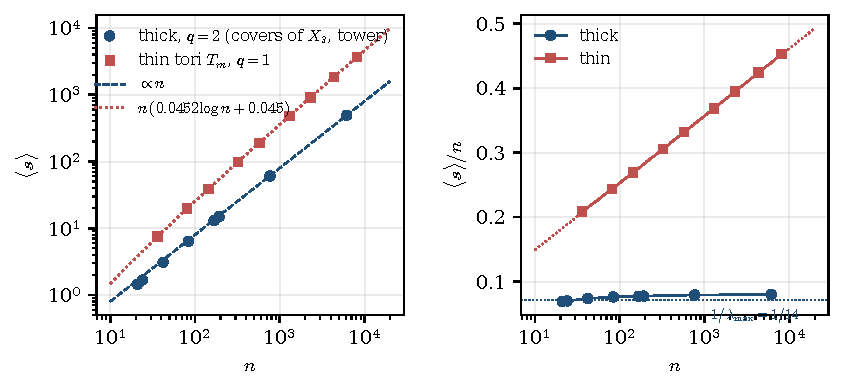
\includegraphics[width=\textwidth]{figures/fig_avalanche_distribution.pdf}
\caption{Exact mean avalanche size $\langle s\rangle=\mathbf 1^{t}G\mathbf 1/(n-1)$ of the vertex
sandpile (sink $=$ vertex $0$, Theorem~\ref{V3P2:thm:mean}), computed by solving the reduced Laplacian
system. Thick, $q=2$: the abelian covers $Y_{21},Y_{24},Y_{42},Y_{84},Y_{168}$ of $X_3$ and the levels
$n=192,768,6144$ of the canonical $2$-tower of Section~\ref{V3P6:sec:cs}. Thin, $q=1$: the tori
$T_m$, $m=6,\dots,90$ ($n=m^{2}$), whose $1$-skeleton is the triangular lattice. Left: $\langle s\rangle$
against $n$ on logarithmic axes, with the line $\propto n$ through the thick family and the fit
$n(a\log n+c)$ through the thin one. Right: $\langle s\rangle/n$, which stays between $0.069$ and $0.080$
on the thick family, as Corollary~\ref{V3P2:cor:linear} predicts ($\ge1/\lambda_{\max}=1/14$), and grows
like $a\log n$ on the thin family, with fitted $a=0.0452$; the triangular-lattice value is
$\sqrt3/(12\pi)=0.0459$, since there $\lambda(k)\approx\frac32|k|^{2}$ and the Brillouin zone has area
$8\pi^{2}/\sqrt3$ (the constant $\frac1{4\pi}$ of Corollary~\ref{V3P2:cor:linear} is that of the square
torus). Drawn by \texttt{code/make\_figures.py}; $\langle s\rangle(Y_{21})=29/20$ is checked there.}
\label{V3P2:fig:avalanche}
\end{figure}

\begin{proposition}[Lyons \cite{Lyons2005}]\label{V3P2:prop:lyons}
If finite $d$-regular graphs $G_j$ converge in the Benjamini--Schramm sense to a transitive
graph $G$, then
$\frac1{|V(G_j)|}\log|\Jac_0(G_j)|\to h(G)=\log d-\sum_{k\ge1}\frac{p_k(o,o)}{k}$, where
$p_k(o,o)$ is the $k$-step return probability of simple random walk on $G$.
\end{proposition}

For quotients $\Gamma_j\backslash B$ with injectivity radius tending to infinity, the limit
graph is the $1$-skeleton of the building. It is transitive, because the Cartwright--Mantero--Steger--Zappa
group acts simply transitively on vertices (Vol.~I--II, Construction~\ref{M-X:con:thick}).
Its entropy $h(B^{(1)})<\log(2(q^{2}+q+1))$ is the ``asymptotic principal exponent'' of the
vertex sandpile groups. We do not compute it. The finite complexes of this volume form a
bounded chain, not a Benjamini--Schramm sequence, and their values
(Table~\ref{V3P2:tab:covers}) are finite-size data only.

\section{Scaling: what can and cannot be claimed}\label{V3P2:sec:scaling}

\begin{proposition}[Critical branching \cite{Harris63}]\label{V3P2:prop:gw}
Let $(Z_t)$ be a Galton--Watson process with offspring mean $1$ and variance
$\sigma^{2}\in(0,\infty)$. Then $\mathbb P(Z_t>0)\sim2/(\sigma^{2}t)$. If the offspring law
is aperiodic, the total progeny $S$ satisfies
$\mathbb P(S=s)\sim(2\pi\sigma^{2})^{-1/2}s^{-3/2}$. Conditionally on survival to time $t$,
$Z_t/t$ converges to an exponential law (Yaglom). Hence the size exponent is $\tau=3/2$, the
duration exponent is $\tau_T=2$, and $s\sim T^{2}$.
\end{proposition}

\begin{conjecture}[Mean-field class]\label{V3P2:conj:mf}
Let $(Y_j)$ be finite quotients of a thick $\Atwo$ building of order $q$ with injectivity
radius $\to\infty$ and $\lambda_2(\Delta_0)$ bounded below. Then, in the scaling window, the
vertex-sandpile avalanche size and duration have the mean-field exponents $\tau=3/2$ and
$\tau_T=2$, with $s\sim T^{2}$.
\end{conjecture}

\emph{Heuristic.} The local limit is a transitive graph of exponential growth on which
simple random walk has spectral radius $<1$. A toppling at depth $r$ from the seed reaches,
with high probability, sites whose earlier history it has not influenced, so the avalanche
is locally a branching process. Criticality of the stationary state (mean offspring $1$)
then gives Proposition~\ref{V3P2:prop:gw}. The same reasoning is known to be exact on the
Bethe lattice \cite{DM90}. The $1$-skeleton, however, contains many triangles (the chambers),
so the tree approximation is uncontrolled. We do not claim a proof.

\begin{remark}[Corrections concerning exponents]\label{V3P2:rem:exponents}
(1) \emph{The dynamic exponent $z$.} Here $z$ is defined by $T\sim L^{z}$ with $L$ a linear
size. On expanders the diameter is $\Theta(\log n)$, so no power law in $L$ is meaningful.
The well-defined replacement is the size--duration exponent $\gamma$ in $s\sim T^{\gamma}$,
conjecturally $\gamma=2$. (2) \emph{The comparison value $1.22$.} The one-dimensional BTW
model has no power-law avalanches at all. The value $\tau\approx1.22$ is an early numerical
estimate for the \emph{two}-dimensional BTW model; later estimates range over roughly
$1.2$--$1.3$, and no value is proved. (3) \emph{Topology.} The divergence from Euclidean
lattices is not topological. The vertex sandpile does not see $b_1(Y)=0$: its graph has
first Betti number $|E|-n+1=6n+1$ for $q=2$. What it sees is expansion, and its rigorous
signature is Corollary~\ref{V3P2:cor:linear}: $\langle s\rangle=\Theta(n)$ against
$\Theta(n\log n)$. (4) \emph{Chambers.} There is no avalanche of chambers to renormalize
(Corollary~\ref{V3P2:cor:nonabelian}).
\end{remark}

\section{The example \texorpdfstring{$Y_{21}$}{Y21}}\label{V3P2:sec:example}

\begin{proposition}[$Y_{21}$ is dense]\label{V3P2:prop:k777}
The $1$-skeleton of $Y_{21}$ is the complete tripartite graph $K_{7,7,7}$. Consequently
$\Tr A_1^{3}=3\cdot7^{3}=1029$, and the $196=343-147$ non-chamber $3$-cycles of Chapter~\ref{chap:V3P1}
(Section~\ref{V3P1:sec:examples}) are all the type-increasing triangles of $K_{7,7,7}$ that
are not chambers.
\end{proposition}

\begin{proof}
Each vertex has $q^{2}+q+1=7$ neighbours of each other type, and there are exactly $7$
vertices of each type. So every pair of vertices of different types is adjacent, and every
choice of one vertex of each type gives a type-increasing $3$-cycle.
\end{proof}

\paragraph{Thresholds.} The threshold of site $i$ is $M_{ii}$, and the largest stable height is
$M_{ii}-1$:
\begin{center}
\begin{tabular}{lcccc}
\toprule
& vertex $\Delta_0$ & edge $\Delta_1$ & chamber $\Delta_2$ & Hecke $\DeltaH$\\
\midrule
threshold, general $q$ & $2(q^{2}+q+1)$ & $q+3$ & $3$ & $q^{3}-1$\\
threshold, $q=2$ & $14$ & $5$ & $3$ & $7$\\
neighbours in support & $14$ & $20$ & $3q=6$ & $14$\\
abelian dynamics & yes & no & no & no\\
\bottomrule
\end{tabular}
\end{center}

\paragraph{Groups.} By Smith forms, recomputed and in agreement with
Vol.~I--II, Ch.~\ref{M-chap:X}:
\begin{align*}
\Jac_0(Y_{21})&=\Z/2\oplus(\Z/14)^{15}\oplus\Z/98\oplus\Z/294,\quad
|\Jac_0|=21\cdot14^{18}=3\cdot2^{18}\cdot7^{19},\\
\Jac_1(Y_{21})&=(\Z/2)^{10}\oplus(\Z/14)^{10}\oplus(\Z/98)^{26}\oplus\Z/2058\oplus\Z/18522,\\
\Jac_2(Y_{21})&=(\Z/2)^{13}\oplus(\Z/14)^{15}\oplus\Z/98\oplus\Z/294 .
\end{align*}
Here $|\Jac_0|$ is the spanning-tree count $N^{k-2}\prod_i(N-n_i)^{n_i-1}=21\cdot14^{18}$ of
$K_{7,7,7}$. Moreover $H_2(Y_{21};\Z)\cong\Z^{20}$ has discriminant $3\cdot7^{29}$, and
Theorem~\ref{V3P2:thm:hodge} reads
$|\Jac_1|=21\cdot(3\cdot2^{18}\cdot7^{19})\cdot|\Jac_2|\cdot3\cdot7^{29}=2^{48}\cdot3^{4}\cdot7^{68}$.
The group exponents are $294=2\cdot3\cdot7^{2}$ for $\Jac_0$ and
$18522=2\cdot3^{3}\cdot7^{3}$ for $\Jac_1$.

\paragraph{Avalanches.} The spectrum of $\Delta_0(K_{7,7,7})$ is $0$, $14^{(18)}$, $21^{(2)}$,
and $K_{7,7,7}$ is vertex-transitive. By Theorem~\ref{V3P2:thm:mean},
\[
\langle s\rangle=\frac{21}{20}\Bigl(\frac{18}{14}+\frac{2}{21}\Bigr)=\frac{29}{20}=1.45 ,
\]
confirmed exactly by solving $\widetilde\Delta_0x=\mathbf 1$, and by Monte Carlo
($2\cdot10^{5}$ additions: $1.45006$). This number says nothing about criticality:
$Y_{21}$ is too dense (degree $14$ on $21$ vertices) to host a scaling regime.

\begin{table}[ht]
\centering\small
\renewcommand{\arraystretch}{1.2}
\begin{tabular}{lcccccc}
\toprule
$Y$ & $n$ & $\lambda_2(\Delta_0)$ & $\lambda_{\max}$ & $\langle s\rangle$ & $[n/\lambda_{\max},\,n/\lambda_2]$ & $\frac1n\log|\Jac_0|$\\
\midrule
$Y_{21}$ & 21 & 14 & 21 & $29/20=1.4500$ & $[1.00,\,1.50]$ & 2.407026\\
$Y_{24}$ & 24 & 13 & 21 & $7031/4186=1.6796$ & $[1.14,\,1.85]$ & 2.426183\\
$Y_{42}$ & 42 & 8.417424 & 21 & $489107/157768=3.1002$ & $[2.00,\,4.99]$ & 2.485136\\
$Y_{84}$ & 84 & 8.417424 & 21 & $6.3933$ & $[4.00,\,9.98]$ & 2.532442\\
$Y_{168}$ & 168 & 8.417424 & 21 & $12.9760$ & $[8.00,\,19.96]$ & 2.560221\\
\bottomrule
\end{tabular}
\medskip
\caption{Vertex sandpiles on the covers of Chapter~\ref{chap:V3P1} (sink $=$ vertex $0$). The values of
$\langle s\rangle$ are exact rationals for $n\le42$ and floating point otherwise. The
entropies for $Y_{84},Y_{168}$ agree with the $\Jac_0$ data of Vol.~I--II,
Ch.~\ref{M-chap:X} to six digits. $\lambda_{\max}=21$ throughout: it comes from the
$\omega$-twisted characters $\omega^{\tau}$, with $A_1+A_2$ eigenvalue $2\operatorname{Re}
(7\omega)=-7$. For comparison, $\log14=2.639057$.}
\label{V3P2:tab:covers}
\end{table}

\section{Verification battery}\label{V3P2:sec:battery}

\begin{table}[ht]
\centering\scriptsize
\renewcommand{\arraystretch}{1.2}
\resizebox{\textwidth}{!}{%
\begin{tabular}{lcl}
\toprule
check & complexes & result\\
\midrule
(S) switching to a Z-matrix: $\Delta_0$ yes; $\Delta_1,U_1$ no; $\Delta_2$ no (thick), yes ($T_6$); $\DeltaH_{xy}\DeltaH_{yx}=-q$ & $Y_{21},Y_{24},Y_{42},T_6$ & exact\\
(S') $\Delta_1$: diagonal $q+3$, entries $\{0,\pm1\}$, $20$ neighbours, $0$ inside chambers & $Y_{21}$ & exact\\
(N) two-site non-abelian example; $300$ random stabilizations: $0$ non-terminating, $113$ order-dependent, $294$ negative & $Y_{21}$ & exact / numeric (seed 1)\\
(K) $1$-skeleton $=K_{7,7,7}$; $\Tr A_1^{3}=1029$ & $Y_{21}$ & exact\\
(H) $|\Jac_1|\operatorname{disc}\ker\Delta_1=n|\Jac_0||\Jac_2|\operatorname{disc}H_2$; $\det\Delta_1=|\Jac_1|$ when $b_1=0$ & $Y_{21},Y_{24},T_6$ & exact\\
(D) $\langle s\rangle$ as exact rationals; Monte Carlo on $Y_{21}$ within $0.02$ & $Y_{21},Y_{24},Y_{42}$ & exact / numeric\\
(E) $\frac1n\log|\Jac_0|$ from spectra; agreement with Vol.~I--II, Ch.~\ref{M-chap:X} for $Y_{168}$ & five covers & numeric $10^{-6}$\\
\bottomrule
\end{tabular}}
\medskip
\caption{Checks run by \texttt{code/v3p2\_verify.py}; the complexes are built by
\texttt{code/a2\_common.py}.}
\label{V3P2:tab:battery}
\end{table}

\section{Scope, residue, corrections}\label{V3P2:sec:scope}

\begin{remark}[Solved, open]\label{V3P2:rem:scope}
\emph{Solved:} the sign obstruction for every higher toppling operator on thick complexes,
and its absence for chambers on thin ones; the Hodge factorization of the orders of the
critical groups; exact avalanche means, their spectral bounds, and the $\Theta(n)$ versus
$\Theta(n\log n)$ dichotomy; the structure of $Y_{21}$. \emph{Open:}
(a) Conjecture~\ref{V3P2:conj:mf};
(b) the entropy $h(B^{(1)})$ of the building's $1$-skeleton, computable in principle from
return probabilities through the spherical Hecke algebra of $(A_1,A_2)$;
(c) whether some non-sign-coherent generalization of chip-firing (a choice of firing cone
for a general nonsingular matrix) gives a meaningful dynamical avatar of $\Jac_1$;
(d) a structural (not merely numerical) relation between $\Jac_1$, $\Jac_0\oplus\Jac_2$ and
$H_2(Y;\Z)$ refining Theorem~\ref{V3P2:thm:hodge};
(e) the analogue of Theorem~\ref{V3P2:thm:sign} for $\Atilde d$, where the same $3$-cycles
exist.
\end{remark}

\begin{remark}[Corrections to the proposed programme]\label{V3P2:rem:corrections}
(1) The toppling rules built from $\Delta_1$ and $\Delta_2$ are not sandpiles: under every
orientation they are not abelian (Theorem~\ref{V3P2:thm:sign},
Corollary~\ref{V3P2:cor:nonabelian}). The ``recurrent configuration group
$\operatorname{Pic}_k$'' does not exist for $k=1,2$, and only the algebraic
$\coker\Delta_k$ remains. (2) $\operatorname{Pic}_k\cong\Z^{|S_k|-1}/\operatorname{im}\Delta_k'$
is the vertex statement. For $k=1$ and $b_1=0$, $\coker\Delta_1$ is finite of order
$\det\Delta_1$ with no reduction, and ``$|\operatorname{Pic}_1|=\det'\Delta_1$'' is a
tautology. The substantive statement is Theorem~\ref{V3P2:thm:hodge}. (3) Avalanche exponents
are not provable on finite complexes. $\tau=3/2$, $\tau_T=2$, $s\sim T^{2}$ are proved for the
branching approximation and conjectured for the sandpile; $z$ in the usual sense is undefined
on expanders. (4) The Euclidean value $1.22$ is a numerical estimate for the $2$D (not $1$D)
BTW model. (5) The divergence from Euclidean lattices is spectral (expansion), not
topological: it is Corollary~\ref{V3P2:cor:linear}, and $b_1(Y)=0$ plays no role in it.
(6) ``Local nontrivial toppling thresholds'' for $Y_{21}$ are $14,5,3,7$. The ``asymptotic
principal exponent'' is read as the growth rate of $|\Jac_0|$, which is
$2.4070$ per vertex on $Y_{21}$. Its limit along Benjamini--Schramm sequences is the entropy
of Proposition~\ref{V3P2:prop:lyons}, which is not computed here.
\end{remark}

\section*{Acknowledgement of provenance and caveats}

Unrefereed. The classical inputs are Dhar's theory of recurrent states \cite{Dhar90}, the
limit theorems for critical Galton--Watson processes \cite{Harris63}, Lyons' entropy theorem
\cite{Lyons2005}, and the Bethe-lattice computation \cite{DM90}, which is cited only for the
heuristic. Everything else is proved here or in Chapter~\ref{chap:V3P1}. The complexes are rebuilt by
\texttt{code/a2\_common.py} independently of the scripts of Vol.~I--II; where the data
overlap, they agree. The bibliographic data of \cite{Dhar90,DM90,Harris63} have been checked against Crossref and zbMATH.
